% Ce livre n'a pas beaucoup de page, alors on le « gonfle » artificiellement avec petitlivre
\documentclass[petitlivre]{livrelitt}

\Titre{Mon livre}
\Auteur{Doe, John}
\Contributeur{[pht/Photographie] Carstens-Peters, Glenn \et [ill/Illustrations] François, Pascale et Jean-Luc}
\Categorie{Roman}
\Editeur{Éditions du bois}
\DroitsDAuteur{© John Doe, 2017}
\Isbn{978-0-0000000-0-2}{978-0-0000000-1-9}
\InfoImpression{Imprimerie du Lac, 2017}
\DepotLegal{juillet 2017}

\Resume{Ce livre regroupe des textes libres de droits, glanés ça et là, afin de servir de démonstration pour l'écosystème « livrelitt ». Ce résumé fait lui-même partie de la démonstration.

On peut d'ailleurs constater que les paragraphes multiples sont supportés par cette commande de résumé.}

\DuMemeAuteur{
Mon autre livre

Et pourquoi pas un recueil de poésies…
}

\begin{document}

\begin{dedicace}
À tous les lecteurs

puissent-ils y prendre du plaisir…

À tous les écrivains

puissent-ils exercer leur art avec passion !
\end{dedicace}

\chapter*{Avant-propos}

Les illustrations fournies dans cet exemple sont tirées du site www.image-gratuite.com, et sont propriété de leurs auteurs Pascale et Jean-Luc François.

Notez que cet avant-propos ne sera pas dans le sommaire. Ceci est dû à l'étoile qui se trouve au niveau de la commande \etranger{chapter}.

\chapter{Alain-Fournier, le Grand Meaulnes}

Il arriva chez nous un dimanche de novembre 189…

Je continue à dire « chez nous », bien que la maison ne nous appartienne plus. Nous avons quitté le pays depuis bientôt quinze ans et nous n'y reviendrons certainement jamais.

Nous habitions les bâtiments du Cour Supérieur de Sainte-Agathe. Mon père, que j'appelais M. Seurel, comme les autres élèves, y dirigeait à la fois le Cours supérieur, où l'on préparait le brevet d'instituteur, et le Cours moyen. Ma mère faisait la petite classe.

Une longue maison rouge, avec cinq portes vitrées, sous des vignes vierges, à l'extrémité du bourg ; une cour immense avec préaux et buanderie, qui ouvrait en avant sur le village par un grand portail ; sur le côté nord, la route où donnait une petite grille et qui menait vers La Gare, à trois kilomètres ; au sud et par derrière, des champs, des jardins et des prés qui rejoignaient les faubourgs… tel est le plan sommaire de cette demeure où s'écoulèrent les jours les plus tourmentés et les plus chers de ma vie ? demeure d'où partirent et où revinrent se briser, comme des vagues sur un rocher désert, nos aventures.

Le hasard des « changements », une décision d'inspecteur ou de préfet nous avaient conduits là. Vers la fin des vacances, il y a bien longtemps, une voiture de paysan, qui précédait notre ménage, nous avait déposés, ma mère et moi, devant la petite grille rouillée. Des gamins qui volaient des pêches dans le jardin s'étaient enfuis silencieusement par les trous de la haie… Ma mère, que nous appelions Millie, et qui était bien la ménagère la plus méthodique que j'aie jamais connue, était entrée aussitôt dans les pièces remplies de paille poussiéreuse, et tout de suite elle avait constaté avec désespoir, comma à chaque « déplacement », que nos meubles ne tiendraient jamais dans une maison si mal construite… Elle était sortie pour me confier sa détresse. Tout en me parlant, elle avait essuyé doucement avec son mouchoir ma figure d'enfant noircie par le voyage. Puis elle était rentrée faire le compte de toutes les ouvertures qu'il allait falloir condamner pour rendre le logement habitable… Quant à moi, coiffé d'un grand chapeau de paille à rubans, j'étais resté là, sur le gravier de cette cour étrangère, à attendre, à fureter petitement autour du puits et sous le hangar.

C'est ainsi, du moins, que j'imagine aujourd'hui notre arrivée. Car aussitôt que je veux retrouver le lointain souvenir de cette première soirée d'attente dans notre cour de Sainte-Agathe, déjà ce sont d'autres attentes que je me rappelle ; déjà, les deux mains appuyées aux barreaux du portail, je me vois épiant avec anxiété quelqu'un qui va descendre la grand'rue. Et si j'essaie d'imaginer la première nuit que je dus passer dans ma mansarde, au milieu des greniers du premier étage, déjà ce sont d'autres nuits que je me rappelle ; je ne suis plus seul dans cette chambre ; une grande ombre inquiète et amie passe le long des murs et se promène. Tout ce paysage paisible ? l'école, le champ du père Martin, avec ses trois noyers, le jardin dès quatre heures envahi chaque jour par des femmes en visite ? est à jamais, dans ma mémoire, agité, transformé par la présence de celui qui bouleversa toute notre adolescence et dont la fuite même ne nous a pas laissé de repos. Nous étions pourtant depuis dix ans dans ce pays lorsque Meaulnes arriva.

J'avais quinze ans. C'était un froid dimanche de novembre, le premier jour d'automne qui fît songer à l'hiver. Toute la journée, Millie avait attendu une voiture de La Gare qui devait lui apporter un chapeau pour la mauvaise saison. Le matin, elle avait manqué la messe ; et jusqu'au sermon, assis dans le choeur avec les autres enfants, j'avais regardé anxieusement du côté des cloches, pour la voir entrer avec son chapeau neuf.

Après midi, je dus partir seul à vêpres.

D'ailleurs, me dit-elle, pour me consoler, en brossant de sa main mon costume d'enfant, même s'il était arrivé, ce chapeau, il aurait bien fallu sans doute, que je passe mon dimanche à le refaire.

Souvent nos dimanches d'hiver se passaient ainsi. Dès le matin, mon père s'en allait au loin, sur le bord de quelque étang couvert de brume, pêcher le brochet dans une barque ; et ma mère, retirée jusqu'à la nuit dans sa chambre obscure, rafistolait d'humbles toilettes. Elle s'enfermait ainsi de crainte qu'une dame de ses amies, aussi pauvre qu'elle mais aussi fière, vînt la surprendre. Et moi, les vêpres finies, j'attendais, en lisant dans la froide salle à manger, qu'elle ouvrît la porte pour me montrer comment ça lui allait.

Ce dimanche-là, quelque animation devant l'église me retint dehors après vêpres. Un baptême, sous le porche, avait attroupé des gamins. Sur la place, plusieurs hommes du bourg avaient revêtu leurs vareuses de pompiers ; et, les faisceaux formés, transis et battant la semelle, ils écoutaient Boujardon, le brigadier, s'embrouiller dans la théorie…

\begin{figure}[!p]
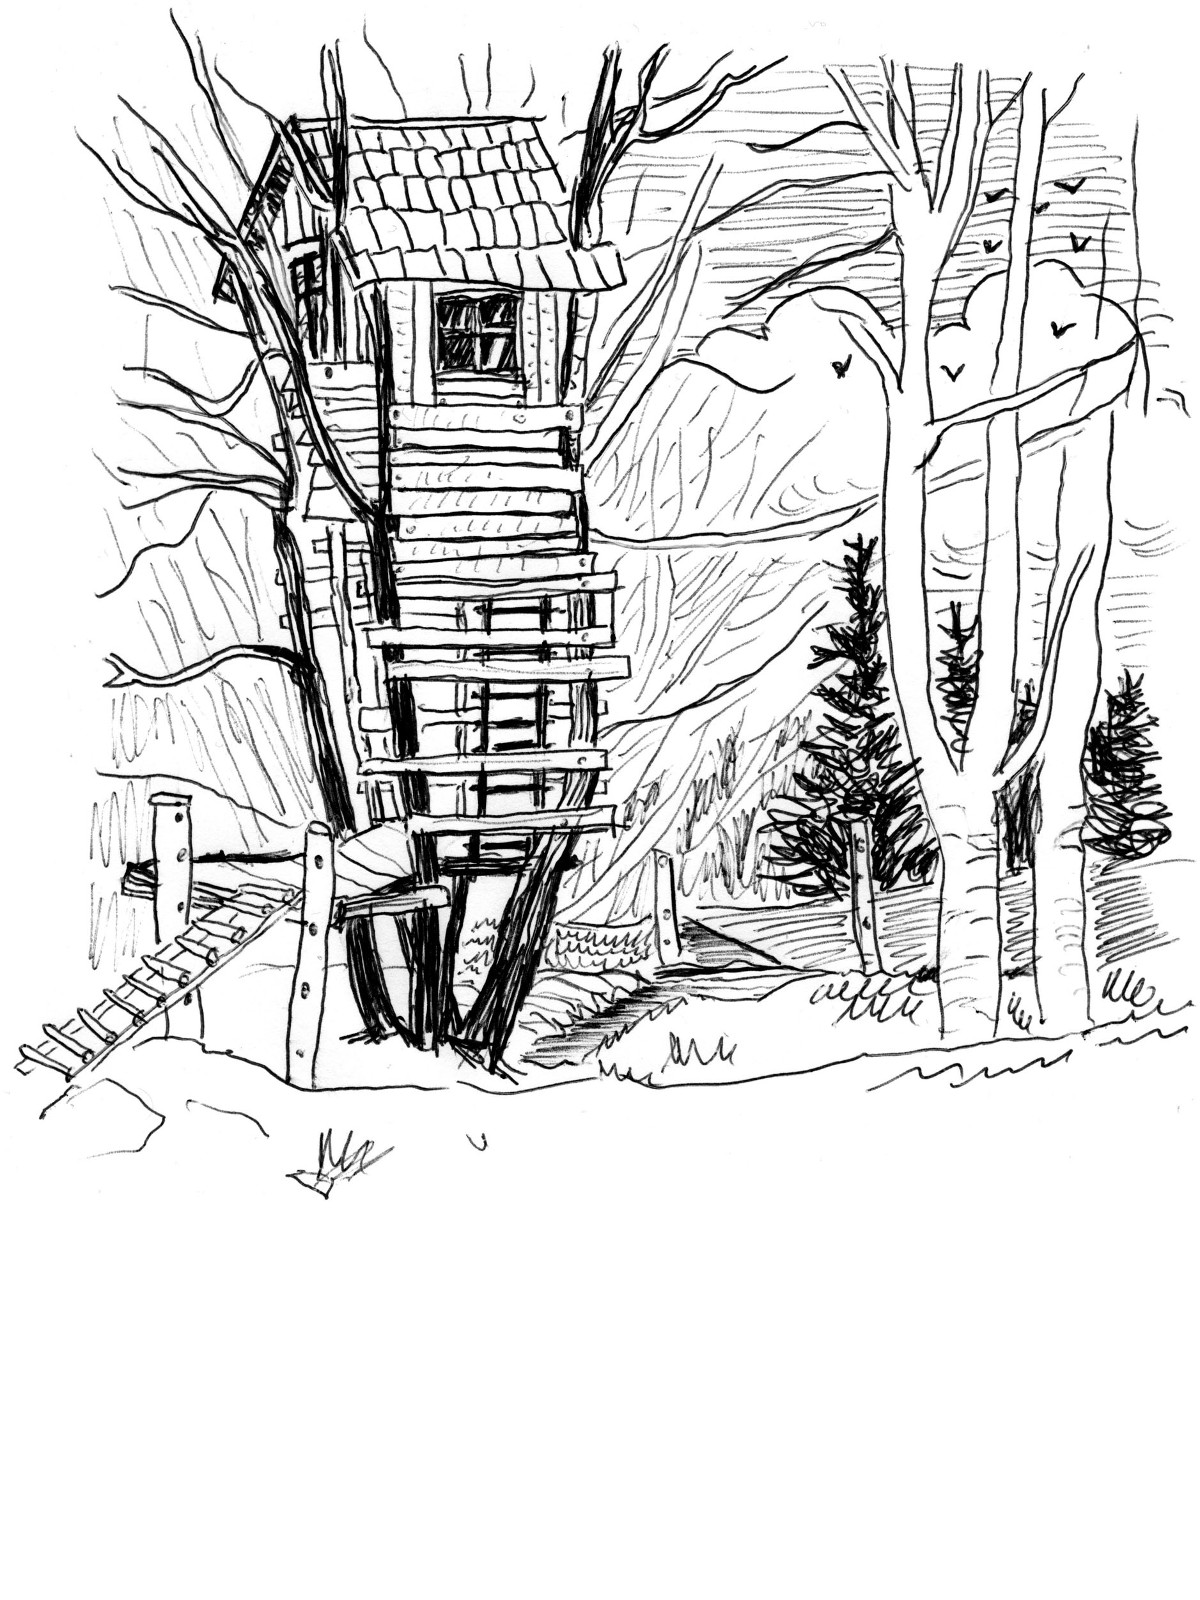
\includegraphics[width=0.9\textwidth]{cabane-dessin.jpg}
\end{figure}

\chapter{Jules Verne, 20 000 lieues sous les mers}

« Eh ! mille diables ! s’écria Ned Land, frappant du pied la tôle sonore, ouvrez donc, navigateurs peu hospitaliers ! »

Mais il était difficile de se faire entendre au milieu des battements assourdissants de l’hélice. Heureusement, le mouvement d’immersion s’arrêta.

Soudain, un bruit de ferrures violemment poussées se produisit à l’intérieur du bateau. Une plaque se souleva, un homme parut, jeta un cri bizarre et disparut aussitôt.

Quelques instants après, huit solides gaillards, le visage voilé, apparaissaient silencieusement, et nous entraînaient dans leur formidable machine.

\separateurpar

Mobilis in mobile

Cet enlèvement, si brutalement exécuté, s’était accompli avec la rapidité de l’éclair. Mes compagnons et moi, nous n’avions pas eu le temps de nous reconnaître. Je ne sais ce qu’ils éprouvèrent en se sentant introduits dans cette prison flottante ; mais, pour mon compte, un rapide frisson me glaça l’épiderme. A qui avions-nous affaire ? Sans doute à quelques pirates d’une nouvelle espèce qui exploitaient la mer à leur façon.

A peine l’étroit panneau fut-il refermé sur moi, qu’une obscurité profonde m’enveloppa. Mes yeux, imprégnés de la lumière extérieure, ne purent rien percevoir. Je sentis mes pieds nus se cramponner aux échelons d’une échelle de fer. Ned Land et Conseil, vigoureusement saisis, me suivaient. Au bas de l’échelle, une porte s’ouvrit et se referma immédiatement sur nous avec un retentissement sonore.

Nous étions seuls. Où ? Je ne pouvais le dire, à peine l’imaginer. Tout était noir, mais d’un noir si absolu, qu’après quelques minutes, mes yeux n’avaient encore pu saisir une de ces lueurs indéterminées qui flottent dans les plus profondes nuits.

Cependant, Ned Land, furieux de ces façons de procéder, donnait un libre cours à son indignation.

« Mille diables ! s’écriait-il, voilà des gens qui en remonteraient aux Calédoniens pour l’hospitalité ! Il ne leur manque plus que d’être anthropophages ! Je n’en serais pas surpris, mais je déclare que l’on ne me mangera pas sans que je proteste !

— Calmez-vous, ami Ned, calmez-vous, répondit tranquillement Conseil. Ne vous emportez pas avant l’heure. Nous ne sommes pas encore dans la rôtissoire !

— Dans la rôtissoire, non, riposta le Canadien, mais dans le four, à coup sûr ! Il y fait assez noir. Heureusement, mon bowie-kniff ne m’a pas quitté, et j’y vois toujours assez clair pour m’en servir. Le premier de ces bandits qui met la main sur moi…

— Ne vous irritez pas, Ned, dis-je alors au harponneur, et ne nous compromettez point par d’inutiles violences. Qui sait si on ne nous écoute pas ! Tâchons plutôt de savoir où nous sommes ! »

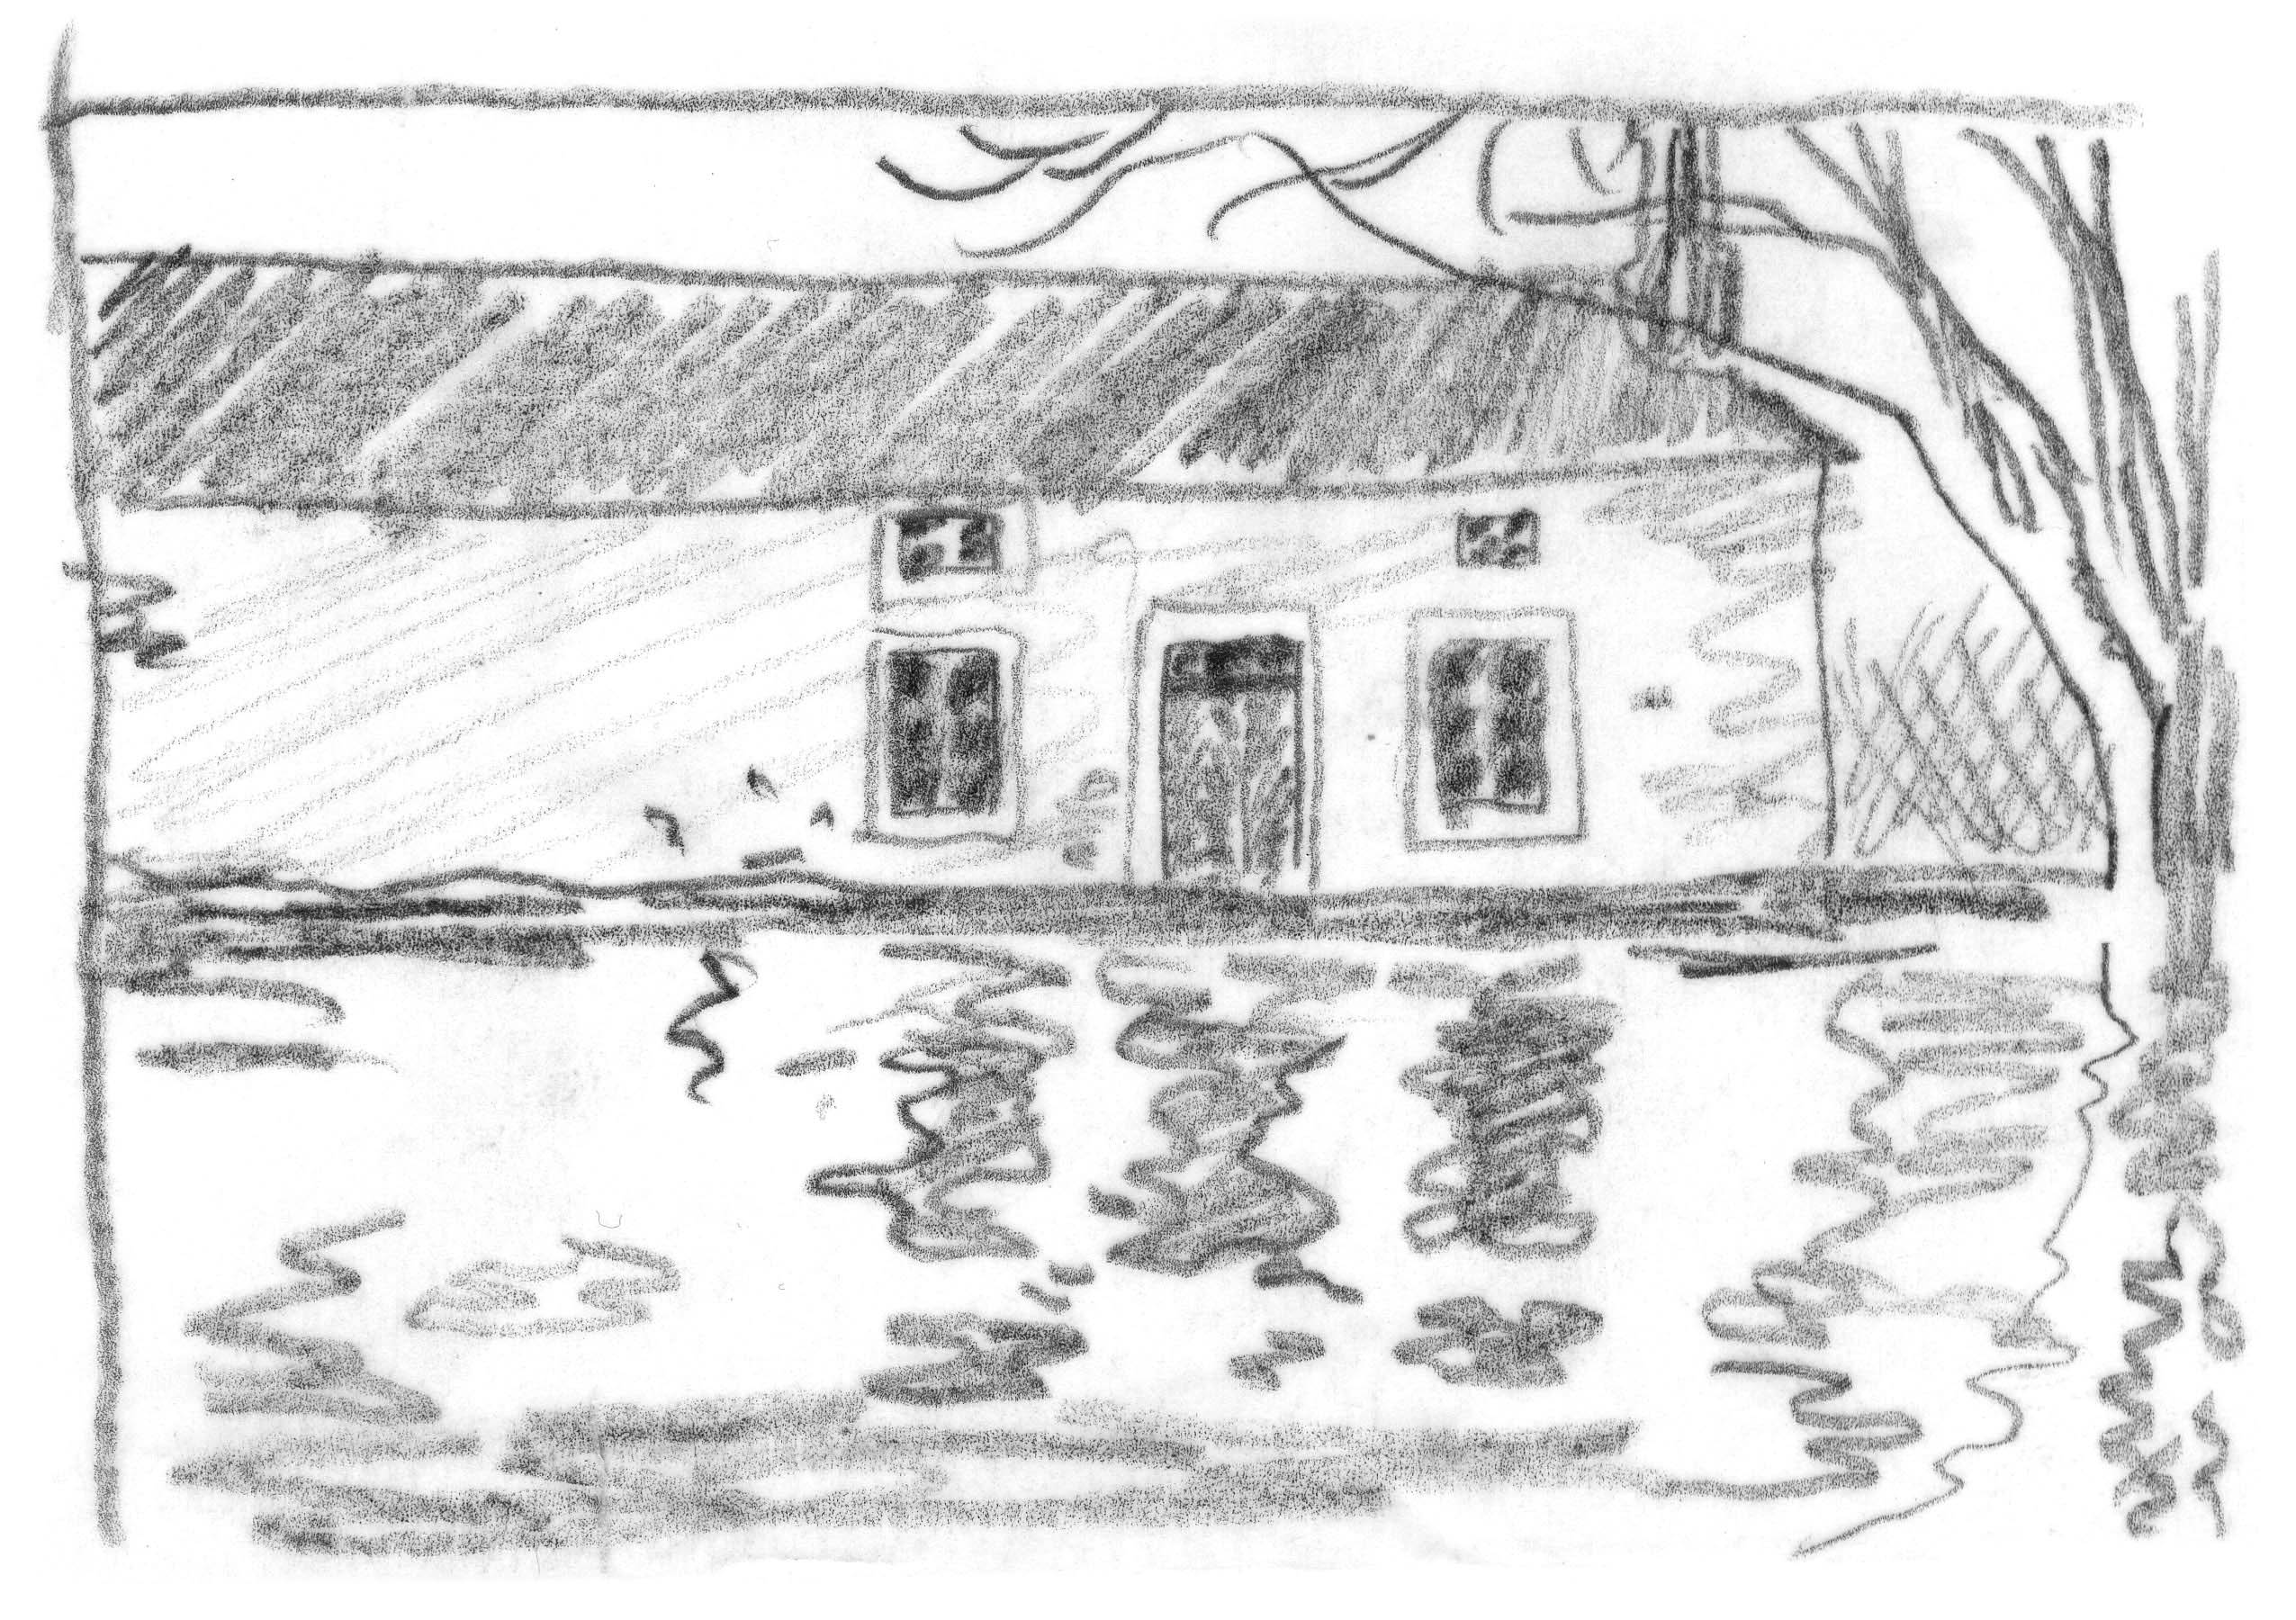
\includegraphics[width=5cm]{maison-etang.jpg}

\tableofcontents

\end{document}
